\chapter[Tecnología GaN HEMT]{Tecnología GaN HEMT} \label{sec:gan_hemt}
\section{Contexto y relevancia de la tecnología del transistor}
La selección del transistor constituye una de las decisiones de diseño con mayor impacto sobre el desempeño global de un amplificador de potencia destinado a aplicaciones CubeSat, ya que de ella dependen simultáneamente la eficiencia, la masa del sistema de disipación térmica y la confiabilidad del enlace en el ambiente orbital. Las restricciones propias de una plataforma nanosatelital, en particular la disponibilidad limitada de potencia eléctrica y el presupuesto de masa acotado, exigieron evaluar tecnologías semiconductoras capaces de entregar una densidad de potencia elevada sin comprometer la eficiencia. En este contexto, el nitruro de galio (GaN) se consolidó como la tecnología candidata para cumplir ese rol, dado que combina una tensión de ruptura elevada, una densidad de corriente superior a la de tecnologías competidoras y una eficiencia adecuada a la aplicación.

% ------------------------------------------------------------------------ %
\section{Principio de funcionamiento y características del transistor GaN HEMT}
Una de las propiedades principales del nitruro de galio es que es un material semiconductor de banda prohibida ancha (\textit{wide bandgap}), que le confiere un conjunto de prestaciones superiores a las de tecnologías convencionales como el silicio (Si) o el arseniuro de galio (GaAs) \cite{boomer2020, mishra2008, deblecker2015}. Esto implica que los portadores deben adquirir una mayor energía para pasar a la banda de conducción que en un material semiconductor normal, como el silicio. De esta propiedad se desprenden tres características fundamentales: una tensión de ruptura considerablemente mayor a la de un semiconductor convencional, la posibilidad de operar a mayores temperaturas y una mayor inmunidad a la radiación \cite{mishra2008, deblecker2015}.

La mayor tensión de ruptura permite, en primera instancia, operar el transistor a tensiones más elevadas lo cual a su vez se traduce en un campo eléctrico crítico mayor, de modo que la velocidad de saturación resulta también más elevada, posibilitando la operación del dispositivo a mayores frecuencias y obtener velocidades de conmutación superiores. La relación entre el campo eléctrico y la velocidad de los portadores se describe, de acuerdo con \cite{taur2021}, mediante la ecuación~\eqref{eq:vel_field}

\begin{equation}
    v(E) = \frac{\mu_n E}{1 + E/E_c}
    \label{eq:vel_field}
\end{equation}

donde $\mu_n$ es la movilidad electrónica de bajo campo, $E$ el campo eléctrico aplicado y $E_c$ el campo eléctrico crítico del material. La ecuación~\eqref{eq:vel_field} muestra que, para campos del orden de $E_c$, la velocidad de los portadores tiende asintóticamente a su valor de saturación $v_{sat}$. Dado que el GaN admite valores de $E_c$ sustancialmente mayores antes de alcanzar la ruptura del material, el dispositivo puede operar con tensiones de drain más elevadas mientras los portadores siguen desplazándose a velocidad de saturación, lo que habilita simultáneamente alta tensión de operación y alta frecuencia de conmutación.

Que los transistores GaN puedan operar a mayores temperaturas se explica entendiendo que, al ser la banda prohibida más ancha, resulta estadísticamente menos probable que los portadores pasen espontáneamente a la banda de conducción por excitación térmica, de modo que el material conserva su comportamiento semiconductor hasta temperaturas más elevadas \cite{deblecker2015}.

El transistor de efecto de campo de alta movilidad electrónica (\textit{High Electron Mobility Transistor}, HEMT) basado en GaN se construye a partir de una heterojuntura entre dos materiales semiconductores de distinta banda prohibida de energía. La estructura típica se crece epitaxialmente sobre un sustrato de silicio (Si), carburo de silicio (SiC) o zafiro, interponiendo una capa fina de nitruro de aluminio (AlN) que actúa como capa semilla para mejorar la calidad cristalina del crecimiento posterior, seguida de una capa de GaN de alta pureza no dopado y, finalmente, una capa barrera delgada de AlGaN con dopaje tipo N \cite{marini2013}. Entre los sustratos mencionados, el SiC se emplea preferentemente en aplicaciones de potencia por su elevada conductividad térmica, factor relevante para la evacuación del calor generado durante la operación del dispositivo.

En la interfaz entre el GaN y el AlGaN se produce una discontinuidad en la banda de conducción que, combinada con los efectos de polarización piezoeléctrica y espontánea propios de la estructura cristalina hexagonal del GaN \cite{ambacher2000}, da origen a un pozo de potencial confinante. Dentro de este pozo se acumula una densidad superficial de carga elevada que constituye el denominado gas bidimensional de electrones (\textit{two-dimensional electron gas}, 2DEG) \cite{mishra2008}. Los terminales del dispositivo, denominados drain, gate y source siguiendo la nomenclatura habitual en inglés, se disponen sobre la superficie de la estructura epitaxial, de modo que el drain y el source contactan eléctricamente al 2DEG, mientras que el gate, ubicado entre ambos, permite modular la conducción del canal.

Debido al confinamiento de los portadores en el pozo de potencial, los electrones del 2DEG solo pueden desplazarse a lo largo de un eje, lo que reduce la dispersión asociada a choques en la estructura cristalina y, en consecuencia, disminuye la resistencia del canal. Adicionalmente, la separación espacial entre los electrones confinados en el canal de GaN y los átomos donores ubicados en la capa barrera de AlGaN reduce sustancialmente la dispersión por impurezas ionizadas, lo que permite alcanzar movilidades electrónicas superiores a las obtenidas en heterojunturas equivalentes de GaAs \cite{mishra2008}. La elevada concentración de portadores del 2DEG, combinada con su movimiento restringido a una sola dirección, incrementa tanto la movilidad electrónica efectiva como la densidad de corriente que el canal es capaz de sostener. La densidad de corriente máxima $J_{D}$ resulta proporcional al producto entre la densidad superficial de carga del 2DEG y la velocidad de saturación de los portadores, de modo que un incremento en cualquiera de estos dos factores eleva directamente la capacidad de corriente del dispositivo sin necesidad de aumentar el área activa.

La combinación de mayores densidades de corriente con la posibilidad de operar a tensiones más elevadas da como resultado un aumento considerable en la densidad de potencia de salida del dispositivo respecto de tecnologías competidoras, alcanzando valores reportados del orden de 40~W/mm² en dispositivos experimentales con field plate doble \cite{wu2006}. Esta característica resulta especialmente relevante en aplicaciones CubeSat, ya que una mayor densidad de potencia implica que, para una potencia de salida dada, el transistor disipa la misma potencia térmica en un área de silicio considerablemente menor, lo que reduce el tamaño y la masa del disipador requerido para mantener la temperatura de juntura dentro de límites admisibles.

Una magnitud adicional que vincula las propiedades del material con el desempeño práctico del dispositivo es la resistencia de canal en conducción (\textit{on-state resistance}, $r_{on}$). En un transistor de efecto de campo de óxido metálico semiconductor (MOSFET) o un HEMT, las pérdidas de conducción dependen esencialmente de la permitividad relativa $\varepsilon_r$ y del campo eléctrico de ruptura $E_c$ del material, de modo que $r_{on}$ resulta inversamente proporcional a ambas magnitudes \cite{deblecker2015}:

\begin{equation}
    r_{on} \propto \frac{1}{\varepsilon_r \, E_c^3}
    \label{eq:ron}
\end{equation}

La ecuación~\eqref{eq:ron} muestra que, dado que el GaN posee un campo de ruptura considerablemente mayor que el del silicio, la resistencia de canal alcanzable para una misma tensión resulta menor, obteniendo así menores pérdidas de conducción y, por lo tanto, en una mayor eficiencia.

Finalmente, una limitación temprana de los GaN HEMT fue la denominada dispersión corriente continua a RF (\textit{DC-to-RF dispersion} o \textit{current collapse}), fenómeno asociado a trampas de carga superficiales y de volumen que reducían la potencia de salida obtenida en condiciones de gran señal respecto de la predicha por las curvas estáticas $I$-$V$ \cite{mishra2008}. La carga atrapada en la región de acceso entre gate y drain da origen a un denominado gate virtual, que modula el 2DEG subyacente e incrementa transitoriamente la resistencia de canal en conducción \cite{mistri2025}.Dos innovaciones permitieron mitigar este efecto: la pasivación superficial mediante nitruro de silicio y la incorporación de field plates \cite{chiang2012}. El field plate consiste en una extensión metálica, conectada eléctricamente al gate o al source, que se superpone parcialmente sobre la región de acceso entre el gate y el drain mediante una capa dieléctrica intermedia. Su función es redistribuir el perfil del campo eléctrico en dicha región para reducir el valor del campo máximo en el borde del gate y desplazando parte de la caída de tensión hacia el borde del field plate \cite{mishra2008}. Esta redistribución incrementa la tensión de ruptura del dispositivo y reduce simultáneamente el efecto de las trampas superficiales sobre la dispersión de potencia, lo que mejora tanto la linealidad como la densidad de potencia obtenible en gran señal \cite{wu2004}.

La Figura~\ref{fig:cross_section_sin_fp} ilustra la sección transversal esquemática de un GaN HEMT convencional, sin field plate, evidenciando la región de acceso entre el gate y el drain donde se concentra el campo eléctrico máximo del dispositivo en ausencia de dicha estructura.

\begin{figure}[H]
    \centering
    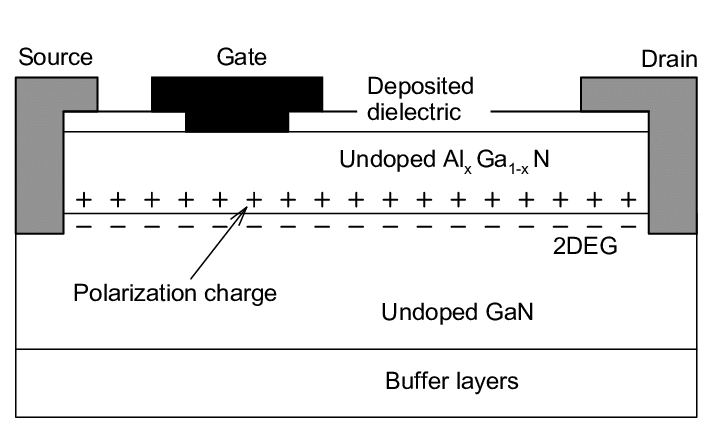
\includegraphics[width=0.6\linewidth]{Figures/crossection_gan.png}
    \caption{Sección transversal esquemática de un GaN HEMT sin field plate \cite{dimitrijev2014}.}
    \label{fig:cross_section_sin_fp}
\end{figure}

Existen dos configuraciones principales: el field plate conectado al gate (\textit{gate-connected field plate}), que introduce una capacitancia adicional gate-drain con la consecuente realimentación de Miller negativa y reducción de la frecuencia de corte, y el field plate conectado al source (\textit{source-connected field plate}), que evita dicha penalización al transformar la capacitancia adicional en una capacitancia drain-source absorbible por la red de salida \cite{mishra2008}. La Figura~\ref{fig:cross_fp} compara esquemáticamente ambas configuraciones.

\begin{figure}[H]
    \centering
    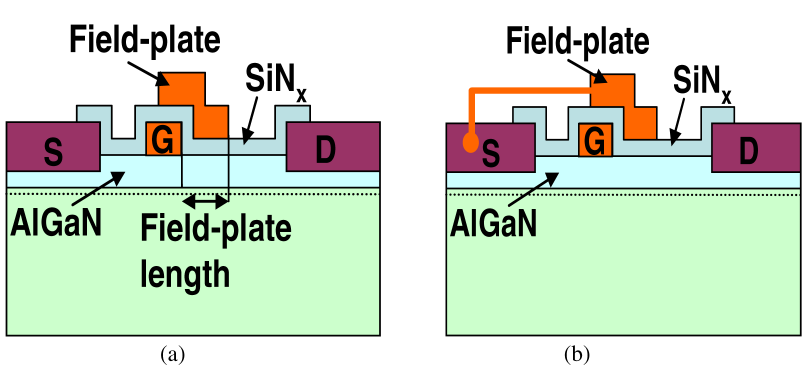
\includegraphics[width=0.85\linewidth]{Figures/fieldplate_gan.png}
    \caption{Sección transversal de las configuraciones de field plate conectado (a) al gate y (b) al source \cite{mishra2008}.}
    \label{fig:cross_fp}
\end{figure}

Asimismo, una característica intrínseca de la mayoría de los GaN HEMT comerciales, es que se fabrican en modo de agotamiento (\textit{depletion mode}), también descripto como dispositivo normalmente encendido. Esto significa que, en ausencia de polarización de gate ($V_{GS}=0$), el 2DEG permanece completo y el canal conduce sin restricción, de modo que el transistor requiere una tensión de gate negativa, para regular o interrumpir la conducción~\cite{Macom}. Esta propiedad de canal permanente introduce un requisito particular en la secuencia de encendido y apagado del circuito de polarización. Si la tensión de drain se aplica antes de que el gate haya alcanzado una tensión suficientemente negativa, el transistor conduce de manera no controlada en el instante en que se energiza el drain, lo que puede dar lugar a corrientes de drain excesivas y al consecuente riesgo de fuga térmica o daño permanente del dispositivo. Por este motivo, la secuencia de polarización recomendada establece que el gate debe alcanzar su tensión de corte antes de aplicar tensión al drain, y que, de manera inversa, el drain debe quedar sin tensión antes de remover la polarización negativa del gate \cite{Macom}.

% ------------------------------------------------------------------------ %
\section{Comparación con tecnologías LDMOS y GaAs}
Dos de las tecnologías más tradicionales y establecidas en la industria de los semiconductores son el silicio difundido lateralmente (\textit{Laterally Diffused Metal Oxide Semiconductor}, LDMOS) y el arseniuro de galio (GaAs). El LDMOS es un transistor de efecto de campo de silicio cuya estructura incorpora una región de drift débilmente dopada entre el canal y el contacto de drain, lo que permite sostener tensiones de drain relativamente elevadas para un dispositivo de silicio. Esta tecnología domina el segmento de estaciones base celulares en bandas de frecuencia bajas, debido a su bajo costo de fabricación y su elevada robustez, aunque su frecuencia de corte y su densidad de potencia resultan insuficientes para aplicaciones de banda S con los requisitos de eficiencia y tamaño que impone una plataforma CubeSat.

El GaAs, por su parte, es un semiconductor compuesto de banda prohibida intermedia entre la del silicio y la del GaN, que se emplea típicamente en transistores pseudomórficos de alta movilidad electrónica (\textit{pseudomorphic HEMT}, pHEMT). Su principal ventaja sobre el silicio es la mayor movilidad electrónica, lo que posibilita una frecuencia de operación más elevada. No obstante, su tensión de ruptura y su densidad de potencia resultan considerablemente menores que las del GaN, lo que obliga a emplear dispositivos de mayor periferia de compuerta para alcanzar una potencia de salida equivalente, con la consecuente penalización en masa y en facilidad de adaptación de impedancias \cite{mishra2008}.

La Figura~\ref{fig:freq_power_materiales} resume gráficamente esta comparación, ubicando a cada tecnología semiconductora según el rango de potencia de RF y la frecuencia de operación característica. Se observa que el silicio, cubre la región de menor frecuencia con niveles de potencia moderados, mientras que el GaAs se extiende hacia frecuencias mayores a costa de una potencia de RF disponible inferior. El GaN, en cambio, ocupa una región claramente desplazada hacia valores simultáneamente mayores de potencia y de frecuencia respecto de ambas tecnologías, ilustrando la motivación expuesta en los párrafos anteriores para su adopción en el presente trabajo. Las regiones correspondientes a SiGe e InP, si bien se incluyen en la figura a modo de referencia comparativa más amplia, corresponden a tecnologías orientadas predominantemente a aplicaciones de muy alta frecuencia con niveles de potencia reducidos, por lo que no constituyen alternativas relevantes para los requisitos de la aplicación considerada.

\begin{figure}[H]
    \centering
    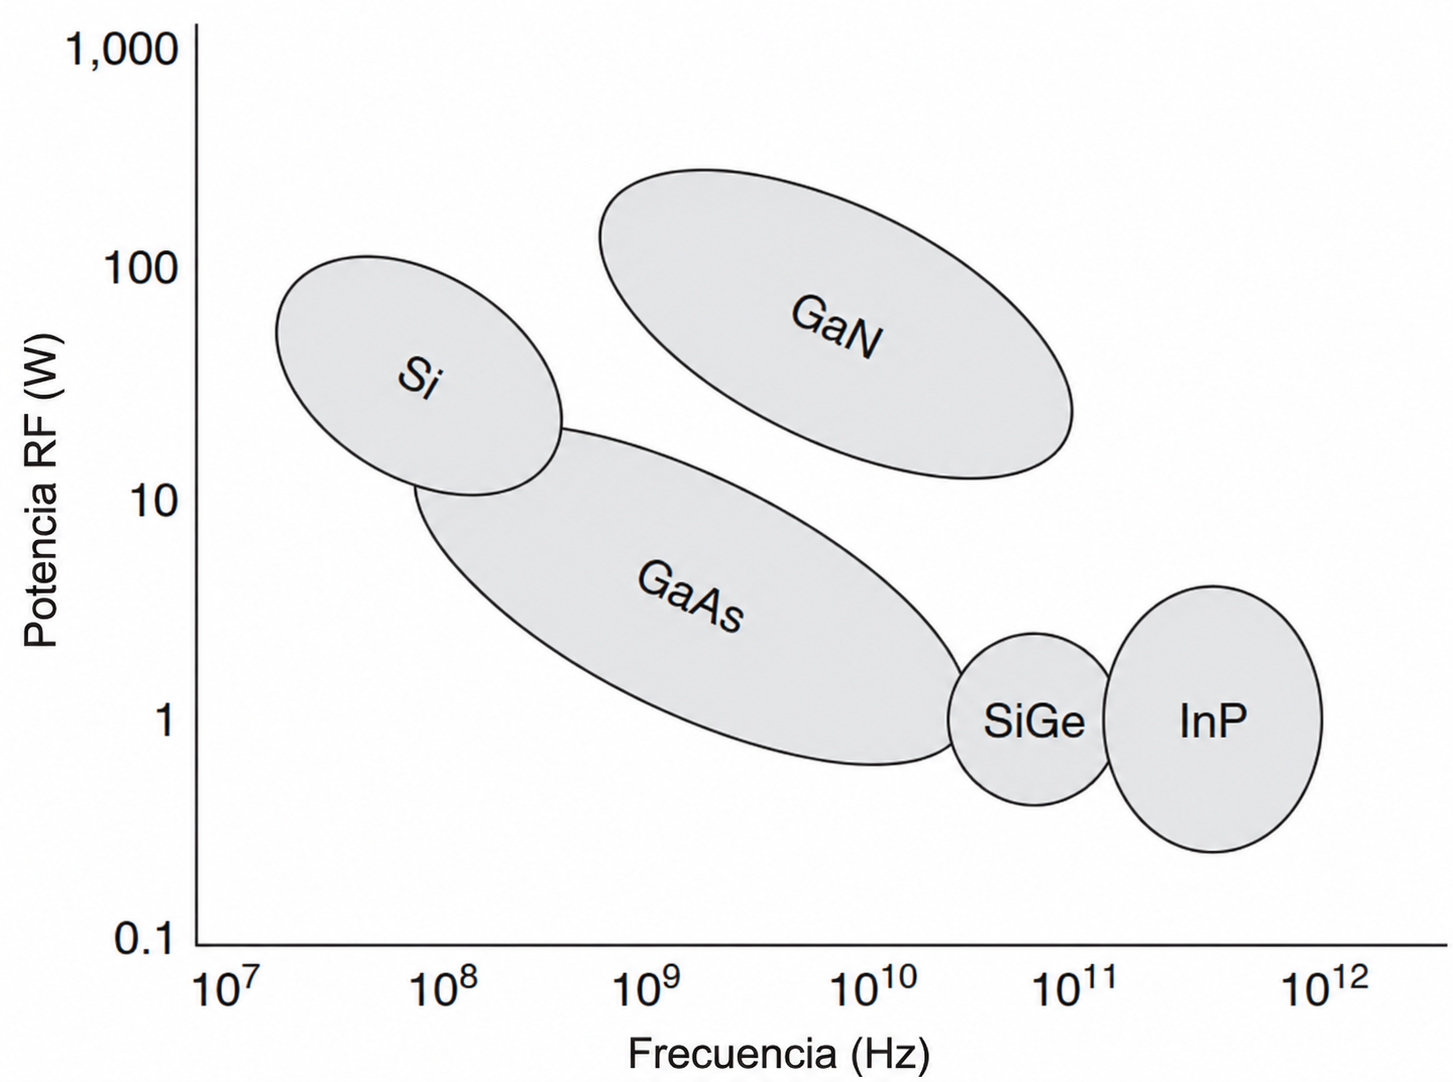
\includegraphics[width=0.65\linewidth]{Figures/transistor_tech_comparison.png}
    \caption{Rangos característicos de potencia de RF y frecuencia de operación alcanzables para distintas tecnologías semiconductoras \cite{bowick2008}.}
    \label{fig:freq_power_materiales}
\end{figure}

En la Tabla~\ref{tab:material_comparison} se resumen las propiedades físicas más relevantes de los materiales semiconductores considerados, a partir de los valores reportados en \cite{mishra2008}.

\begin{table}[H]
    \centering
    \caption{Propiedades físicas comparativas de Si, GaAs y GaN, relacionadas con el desempeño en aplicaciones de potencia de alta frecuencia.}
    \label{tab:material_comparison}
    \begin{tabular}{lcccc}
        \hline\hline
        \textbf{Propiedad}                                 & \textbf{Símbolo} & \textbf{Si} & \textbf{GaAs} & \textbf{GaN} \\
        \hline
        Banda prohibida (eV)                               & $E_g$            & 1,1       & 1,42        & 3,39       \\
        Campo de ruptura (MV/cm)                           & $E_c$            & 0,3       & 0,4         & 3,3        \\
        Movilidad electrónica (cm$^{2}$/V$\cdot$s)         & $\mu_n$          & 1350      & 8500        & 1200       \\
        Velocidad de saturación ($\times 10^7$ cm/s)       & $v_{sat}$        & 1,0       & 1,0         & 2,5        \\
        Conductividad térmica (W/cm$\cdot$K)               & $\Theta$         & 1,5       & 0,43        & 1,3        \\
        Conc. intrínseca de portadores (cm$^{-3}$) & $n_i$ & $1{,}5\times10^{10}$ & $1{,}5\times10^{6}$ & $1{,}9\times10^{-10}$ \\ 
        \hline\hline
    \end{tabular}
\end{table}

\subsection{Figura de mérito de Johnson}
A fin de comparar cuantitativamente el potencial de los distintos materiales semiconductores para aplicaciones simultáneas de alta frecuencia y alta potencia, Johnson propuso una figura de mérito (\textit{Johnson Figure of Merit}, JFM) derivada del producto entre el campo eléctrico de ruptura $E_c$ y la velocidad de saturación de los portadores $v_{sat}$ \cite{johnson1965}

\begin{equation}
    \mathrm{JM} = \left( \frac{E_c \, v_{sat}}{2\pi} \right)^2
    \label{eq:jfm}
\end{equation}

En la ecuación~\eqref{eq:jfm}, $E_c$ se expresa en V/cm y $v_{sat}$ en cm/s, de modo que el resultado posee unidades de potencia al cuadrado sobre frecuencia al cuadrado, lo que permite interpretar a la JFM como un límite superior del producto entre la potencia y la frecuencia de operación que un transistor construido con ese material puede alcanzar. Esta magnitud surge de considerar que la máxima tensión que puede soportar el dispositivo está acotada por $E_c$, mientras que la máxima frecuencia de conmutación está acotada por el tiempo de tránsito de los portadores a través de la región activa, tiempo que depende inversamente de $v_{sat}$. Al evaluar la ecuación~\eqref{eq:jfm} para los materiales de la Tabla~\ref{tab:material_comparison} y normalizar los resultados respecto del silicio, se obtienen valores de JFM relativa de 2{,}7 para el GaAs, 20 para el 4H-SiC y 27{,}5 para el GaN \cite{mishra2008}. Esta diferencia de más de un orden de magnitud respecto del silicio, y de un factor cercano a 10 respecto del GaAs, proporciona una justificación cuantitativa adicional para la selección de GaN como tecnología del transistor de potencia de este trabajo.

\subsection{Tolerancia a la radiación}
Además de las ventajas en tensión de ruptura, densidad de potencia y temperatura de operación descriptas anteriormente, la inmunidad a la radiación del GaN HEMT resulta particularmente relevante para la aplicación CubeSat considerada en este trabajo, dado que el amplificador de potencia opera en un ambiente orbital sometido a bombardeo constante de radiación gamma, neutrones e iones pesados \cite{epcspace2022}.

Ante radiación gamma, un MOSFET de silicio convencional sufre un desplazamiento de la tensión de umbral $V_{th}$ debido a que los fotones de alta energía liberan electrones del óxido de gate, dejando cargas positivas atrapadas que desplazan al dispositivo hacia un estado normalmente encendido. Es decir, un dispositivo construido para operar en \textit{enhancement mode} pasa a trabajar en \textit{depletion mode}. En el GaN HEMT, el gate se encuentra separado del canal por una capa de AlGaN en lugar de un óxido, capa que no acumula carga significativa bajo este tipo de radiación, de modo que el dispositivo conserva sus características eléctricas incluso ante dosis totales ionizantes elevadas \cite{epcspace2022}.

Frente a radiación de neutrones, el mecanismo de falla dominante es el daño por desplazamiento atómico, en el cual partículas de alta energía dispersan átomos de la red cristalina y generan defectos puntuales. Dado que la energía de desplazamiento de un material resulta proporcional a la energía de enlace de sus átomos constituyentes, y que el enlace Ga-N es considerablemente más fuerte que el enlace Si-Si, el GaN presenta una energía de desplazamiento sustancialmente mayor que la del silicio, lo que se traduce en una degradación mínima del dispositivo ante fluencias de neutrones elevadas \cite{epcspace2022}.

Finalmente, ante el impacto de iones pesados, los MOSFET de silicio son susceptibles a dos mecanismos de falla: la ruptura del óxido de gate por el campo eléctrico transitorio inducido por la partícula (\textit{single event gate rupture}) y el cortocircuito momentáneo entre drain y source originado por la nube de pares hueco-electrón generada al atravesar la región de drift (\textit{single event burnout} o \textit{upset}). El GaN HEMT, al carecer de óxido de gate y al no sostener una conducción eficiente de huecos, resulta inherentemente inmune a ambos mecanismos, aunque puede presentar un incremento gradual de la corriente de fuga entre drain y source a medida que se acumula daño por desplazamiento \cite{epcspace2022}.

Los tres mecanismos descriptos dependen de la estructura general del HEMT de GaN, en particular de la ausencia de un óxido de gate y de la baja capacidad de conducción de huecos, y de las propiedades intrínsecas del material, por lo que resultan aplicables tanto a dispositivos en modo de agotamiento como en modo de enriquecimiento. Cabe aclarar, sin embargo, que los valores cuantitativos reportados en la bibliografía corresponden a ensayos realizados sobre dispositivos comerciales en modo de enriquecimiento, por lo que su extrapolación directa al transistor en modo de agotamiento empleado en este trabajo debe considerarse con cautela.

Esta combinación de tolerancia a dosis totales ionizantes elevadas y de inmunidad a eventos únicos inducidos por iones pesados, sumada a las ventajas ya expuestas en materia de eficiencia y densidad de potencia, refuerza la selección de GaN como tecnología del transistor para la presente aplicación satelital.